\chapter{Deep Learning Background}
\label{ch:background}

In this chapter, we review the mathematical foundations for the methods used in this dissertation. We start of with a walk-through in the world of machine learning (section \ref{sec:ml}) and neural networks (section \ref{sec:nn}), after which we expand on the concept of \acrlong{rl} in section \ref{sec:rl}. These \acrlong{ml} methods are combined into a bigger concept, namely deep \acrlong{rl}.

\section{Machine Learning}
\label{sec:ml}
Machine learning is a family of methods used to perform automatic data analysis gaining insight by finding patterns without having to be explicitly programmed. Due to the incredible growth of data everywhere, machine learning methods are booming in many fields, one of them being \gls{ai}.

Machine learning problems have been classified into three categories, from which hybrids are possible:
\begin{itemize}
\item \textbf{Supervised learning.} The machine has access to labeled data. The labels are true solutions from practice mapped from the given input.
\item \textbf{Unsupervised learning.} In this case, we have no access to labeled data, and the goal is to find some sort of structure in the data points, which we call clusters. 
\item \textbf{Reinforcement learning.} An agent has the task to discover an environment. The environment returns feedback signals (rewards and punishments) to the agent. The goal of the program is to find out how the agent can maximize its rewards. We will dive deeper into this topic in section \ref{sec:rl}.
\end{itemize}

\subsection*{Supervised Learning}
In a supervised learning model, we have access to a dataset $\{(x_1,y_1),\cdots,(x_N,y_N)\}$, with $x_i\in\mathcal{X}$ a feature vector and $y_i\in\mathcal{Y}$ the label corresponding to $x_i$. With the model, we associate a function $f:\mathcal{X}\times\mathcal{W}\mapsto\mathcal{Y}$ with $w \in \mathcal{W}$ denoted as the parameters or weights of the model. This function maps input data to a new label. The goal of a supervised learning algorithm is then to optimize the weights in such a way to minimize a certain loss function $L:\mathcal{Y}\times\mathcal{Y}\mapsto\mathbb{R}_{\leq0}$. In regression problems, where we want to estimate for every new data point $x_i$ a label $\hat{y}_i=f(x_i,w)$, the most common loss function is the \gls{mse}:

\begin{equation}
L=\frac{1}{N}\sum_{i=1}^{N}\left(\hat{y}_i-y_i\right)^2
\label{eq:mse}
\end{equation}

By using a learning algorithm, we try to minimize the loss over the dataset. We then hope that the dataset was a good and diverse representation, such that $f$ generalized well to the real world.\\

Here, we will use combinations of supervised and reinforcement learning to let the computer analyze how chess play can be improved. The data will be collected by an agent in the chess environment, and a supervised learning algorithm can be used on this data.

\section{Neural Network}
\label{sec:nn}

A \acrlong{nn} is a mathematical model typically used in \gls{ml} tasks. The model describes how data points are converted into a class label (in case of classification) or a real value (regression). Then a supervised or unsupervised learning algorithm is applied to a dataset. This learning algorithm tunes the variables in the model in such a way, that it minimizes a certain cost or loss function. In case of supervised (which is what we will use to the highest degree in this thesis), this loss function is a measure of error between the output of the model and a true value from the dataset corresponding with the input. These true values can be seen as the target of the model to reach, as described in section \ref{sec:ml}. \\
Neural networks are a supervised learning model constructed in such a way that they more or less imitate the series of interconnected neurons in the human brain, with the philosophy to let a machine solve recognition and decision tasks in the same fashion as a human being would. We will use this model to estimate the static evaluation function of a chess position.\\

\subsection{Feedforward Neural Network}
\label{subsubsec:ann}

\subsubsection*{Feedforward Propagation}
An \gls{ann} is a \gls{nn} in its most general form, where all nodes in the network can be connected. An \gls{fnn} is an \gls{ann} without the possibility of loops and cycles, as shown schematically in figure \ref{fig:nn}. The computation of the output vector of a given input is called feedforward propagation. Inputs are fed linearly via a series of weights to every node in the first layer. The linear combination of inputs then undergoes a nonlinear transformation called the activation, which at its turn is fed forward into all the layers of the next node and so on and so forth up until the output layer. Nodes in the hidden layer are called hidden units, and are slackly analogous to axons in the human brain. The variables of this model are the weights of the linear combinations, every edge thus corresponds to a tunable parameter. \\


\begin{figure}[htbp]
\begin{center}
\begin{tikzpicture}[scale=1.3]
% 1st column
\node               at (0,0) {};
\node[state] (n0_1) at (0,1) {};
\node		 (n0_2) at (0,2) {$\vdots$};
\node[state] (n0_3) at (0,3) {};
\node		 (n0_4) at (0,4) {$\vdots$};
\node[state] (n0_5) at (0,5) {};
\node               at (0,6) {};
% 2nd column
\node[state] (n2_0) at (2,0) {} 		edge[mainedge] (n0_1) edge[mainedge] (n0_3) edge[mainedge] (n0_5);
\node		 (n2_1) at (2,1) {$\vdots$};
\node[state] (n2_2) at (2,2) {} 		edge[mainedge] (n0_1) edge[mainedge] (n0_3) edge[mainedge] (n0_5);
\node		 (n2_3) at (2,3) {$\vdots$};
\node[state] (n2_4) at (2,4) {} 		edge[mainedge] (n0_1) edge[mainedge] (n0_3) edge[mainedge] (n0_5);
\node               at (2,5) {$\vdots$};
\node[state] (n2_6) at (2,6) {} 		edge[mainedge] (n0_1) edge[mainedge] (n0_3) edge[mainedge] (n0_5);
% 3th column
\node		 (n3_0) at (3,0) {};
\node		 (n3_2) at (3,2) {};
\node		 (n3_4) at (3,4) {};
\node		 (n3_6) at (3,6) {};
% 5th column
\node		 (n5_0) at (5,0) {}	edge[mainedge] (n3_0);
\node		 (n5_2) at (5,2) {}	edge[mainedge] (n3_2);
\node		 (n5_4) at (5,4) {}	edge[mainedge] (n3_4);
\node		 (n5_6) at (5,6) {}	edge[mainedge] (n3_6);
% 6th column
\node[state] (n6_0) at (6,0) {};
\node		 (n6_1) at (6,1) {$\vdots$};
\node[state] (n6_2) at (6,2) {};
\node		 (n6_3) at (6,3) {$\vdots$};
\node[state] (n6_4) at (6,4) {};
\node               at (6,5) {$\vdots$};
\node[state] (n6_6) at (6,6) {};
% 6th column
\node[state] (n8_0) at (8,0) {} edge[mainedge] (n6_0) edge[mainedge] (n6_2) edge[mainedge] (n6_4) edge[mainedge] (n6_6);
\node		 (n8_1) at (8,1) {$\vdots$};
\node[state] (n8_2) at (8,2) {}edge[mainedge] (n6_0) edge[mainedge] (n6_2) edge[mainedge] (n6_4)  edge[mainedge] (n6_6);
\node		 (n8_3) at (8,3) {$\vdots$};
\node[state] (n8_4) at (8,4) {}edge[mainedge] (n6_0) edge[mainedge] (n6_2) edge[mainedge] (n6_4)  edge[mainedge] (n6_6);				
\node               at (8,5) {$\vdots$};
\node[state] (n8_6) at (8,6) {}edge[mainedge] (n6_0) edge[mainedge] (n6_2) edge[mainedge] (n6_4)  edge[mainedge] (n6_6);
% 8th column
\node[state] (n10_1) at (10,1) {} edge[mainedge] (n8_0) edge[mainedge] (n8_2) edge[mainedge] (n8_4) edge[mainedge] (n8_6);
\node		 (n10_3) at (10,3) {$\vdots$};
\node[state] (n10_5) at (10,5) {} edge[mainedge] (n8_0) edge[mainedge] (n8_2) edge[mainedge] (n8_4) edge[mainedge] (n8_6);
% Info
\node[] at (0,-1) {Input Layer};
\node[] at (10,-1) {Output Layer};
\node[] at (5,-1) {Hidden Layers};
\node[] at (-1,3) {$\mathbf{s}$};
\node[] at (11,3) {$\mathbf{v}$};
\node[] at (0.75,6) {$\mathbf{W}^{(0)}$};
\node[] at (7,6.5) {$\mathbf{W}^{(M-1)}$};
\node[] at (9.25,6) {$\mathbf{W}^{(M)}$};
\draw [decorate,decoration={brace,amplitude=5pt},yshift=-15pt] (8,0) -- (2,0);
\draw [decorate,decoration={brace,amplitude=5pt},xshift=-15pt] (0,1) -- (0,5);
\draw [decorate,decoration={brace,amplitude=5pt},xshift=15pt] (10,5) -- (10,1);
\end{tikzpicture}
\end{center}
\caption[General \gls{fnn} architecture]{The general architecture of an \gls{fnn}, also called an \gls{fcn} in literature.}
\label{fig:nn}
\end{figure}

Suppose we have $\mathbf{s}=(s_1,s_2,\dotsc,s_D)$ as input vector, the resulting activation at a node $n \in \{1,\dotsc,N_1\}$ in the first hidden layer is then

\begin{equation}
a^{(1)}_n = \sum_{d=1}^{D} w^{(0)}_{dm} s_d
\end{equation}

where $w^{(0)}_{dm}$ represents the weight between input node $s_d$ and hidden unit $a_n$. We can rewrite all activation equations into matrix form with

\begin{equation}
\mathbf{a}^{(1)}=\mathbf{W}^{(0)^{\mathbf{T}}} \mathbf{s}
\end{equation}

where $\mathbf{W}^{(0)}_{dm}=w^{(0)}_{dm}$. If we call the nonlinear transformation of the activation $\sigma(a)$, the output of every hidden unit yields

\begin{align}
z^{(1)}_{n} &= \sigma (a^{(1)}_{n}) \\
	  &= \sigma \left(\sum_{d=1}^{D} w^{(0)}_{dm} s_d\right)
\end{align}

so we obtain the matrix equation
\begin{equation}
\mathbf{z}^{(1)}=\sigma \left(\mathbf{W}^{(0)^{\mathbf{T}}} \mathbf{s}\right)
\end{equation}

By introducing an additional bias vector at the first layer, allowing translation of every activation function to the desired position, we obtain
\begin{equation}
\mathbf{z}^{(1)}=\sigma \left(\mathbf{W}^{(0)^{\mathbf{T}}} \mathbf{s} + \mathbf{b^{(0)}}\right)
\end{equation}

These calculations are performed in a chain-wise fashion, the outputs of the hidden units in every layer are propagated forward until we arrive at the output layer. Hence, for an arbitrary layer \textit{k}, the the activation equation looks like this (Figure \ref{fig:hu}):
\begin{equation}
\mathbf{z}^{(k)}=\sigma \left(\mathbf{W}^{(k-1)^{\mathbf{T}}} \mathbf{s} + \mathbf{b}^{(k-1)}\right)
\end{equation}

\begin{figure}
\centering
\begin{tikzpicture}
% 1st column
\node        (n0_m2)at (0,-2) {};
\node		 		 at (0,-1) {$\vdots$};
\node		 (n0_0) at (0,0) {};
\node		 		 at (0,1) {$\vdots$};
\node		 (n0_2) at (0,2) {};

% 2nd column
\node[state_small] (n2_0) at (2,0) {$+$} 		edge[mainedge] (n0_m2) edge[mainedge] (n0_0) edge[mainedge] (n0_2);

% 3th column
\node[state_small] (n4_0) at (4,0) {$\sigma$} 		edge[mainedge] (n2_0);

% 4th column
\node		 (n6_0) at (6,0) {} edge[mainedge] (n4_0);

\node at (1.5,-1.5) {$\mathbf{W}^{(k-1)}_m$};
\node at (3,0.5) {$a^{(k)}_m$};
\node at (5,0.5) {$z^{(k)}_m$};

\end{tikzpicture}
\caption[Hidden units]{Hidden unit}
\label{fig:hu}
\end{figure}

The final nonlinear equation describing the feedforward propagation of an \gls{nn} is (supposing we have $M$ hidden layers in total)
\begin{equation}
\mathbf{\hat{v}}=\sigma \left(\mathbf{W}^{(M)^{\mathbf{T}}} \mathbf{s} + \mathbf{b}^{(M)}\right)
\end{equation}

which is the estimate of a value from the gls{NN}, given an input sample.

\subsubsection*{Nonlinearity}
Generally, we want the nonlinear transformation of the activation to be some sort of threshold function (mimicking the biological decision of a neuron to let the information propagate further), but most importantly, it should be a differentiable function. This is because the most commonly used learning algorithm, backpropagation, uses differentiation in its optimization of the \gls{nn}. Due to the recursive nature of the network function and backpropagation, we want the derivative of the activation function to be simple as well. Common choices are the sigmoid, tanh and \gls{relu} function. They are compared in \ref{tab:nonlin}. From these functions, the \gls{relu} seems to provide the best performances in most practical examples \cite{mishkin16}. It should be mentioned that some alternatives like the noisy and leaky \gls{relu} can be used with some success \cite{vinod10,maas14}.

\begin{table}[]
\centering
\begin{tabular}{m{2cm} m{2cm} m{4cm} m{2cm}}
\toprule
\textbf{name} & $\sigma (a)$ & $\sigma'(a)$ & \textbf{chart} \\
\midrule
sigmoid & $\frac{1}{1+e^{-a}}$ & $\sigma(a)(1-\sigma(a))$  &  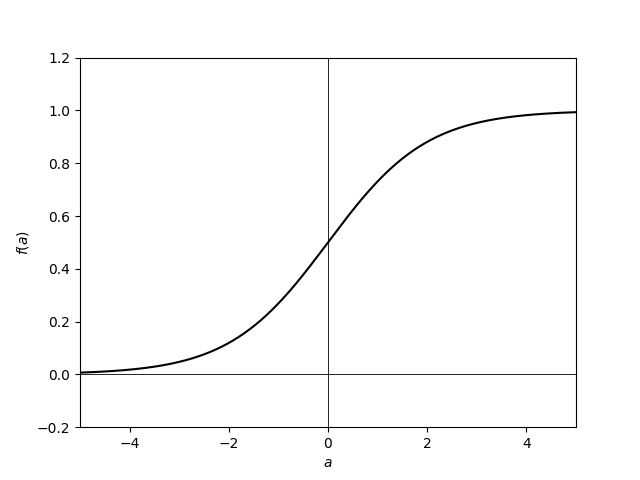
\includegraphics[width=1in]{fig/sigmoid}  \\
tanh & $\tanh(a)$ & $1-\tanh(a)^{2}$&  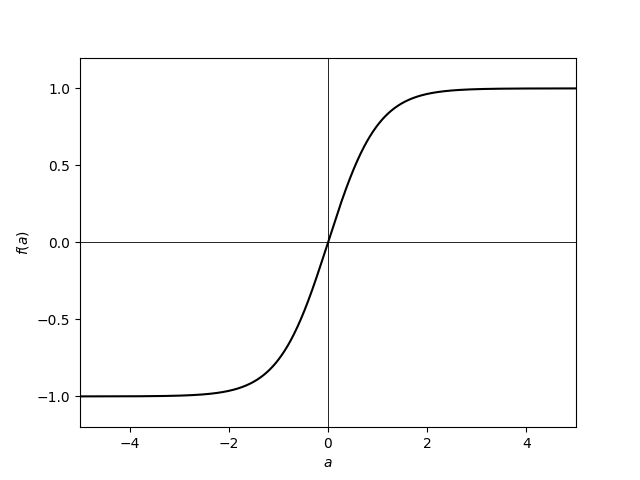
\includegraphics[width=1in]{fig/tanh}        \\
ReLU & $\max(a,0) $ & 
$
  \begin{cases} 
   1 & \text{if } a > 0 \\
   0       & \text{if } a \leq 0
  \end{cases}
$      &  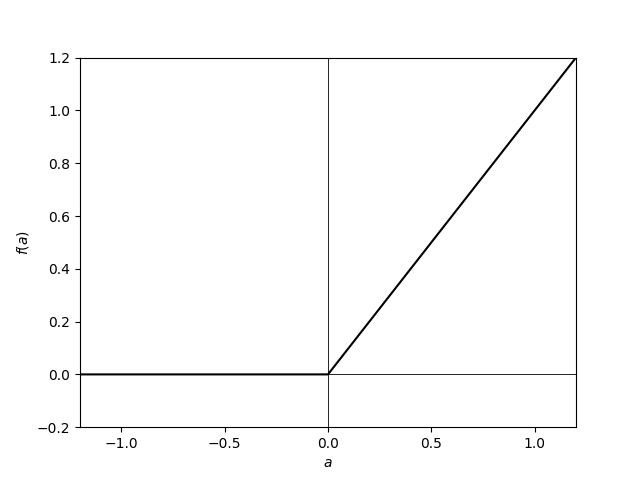
\includegraphics[width=1in]{fig/relu}          \\
\bottomrule
\end{tabular}
\caption[Comparison between activation functions]{Comparison between activation functions}
\label{tab:nonlin}
\end{table}

\subsubsection*{Learning Algorithm}
The goal of the learning algorithm is to tune all model parameters (the weights and bias) such that a global loss function on the training data is minimized. Supposing we have $N$ data samples available, we write 
\begin{equation}
L(w)=\frac{1}{N} \sum_{i=1}^{N} L_i(w)
\end{equation}

so we want to minimize the sum of all errors on all individual samples. The choice of $L_i(w)$ depends on the chosen problem.\\
To find a local optimum, most researchers use gradient descent, a first-order iterative optimization algorithm. It may not find the global optimum, but it is computationally efficient, because of the ease at finding the first partial derivatives of all weights with backpropagation. By updating the weights in the direction of the steepest descent (the gradient of the loss function with respect to all parameters) at each iteration, we gradually reduce the global loss.
\begin{align}
w &\leftarrow w-\alpha\nabla L(w) \\
&=w-\alpha\sum_{i=1}^{N}\frac{\nabla_w L_i(w)}{N}
\end{align}

We observe the introduction of a new training parameter, the step size in the steepest direct also called the learning rate $\alpha$. It should be chosen wisely. The higher the learning rate, the faster the model will learn a local optimum, but if it is too big it might oscillate around the ravine. In contrast, the learning algorithm will be slower but more accurate for a smaller step size. \\
As our problem to approximate the static evaluation function of a chess position is a regression problem, we will use the \gls{mse} from section \ref{sec:ml}. By calculating the derivative we find the update rule for the weights to be

\begin{align}
w&\leftarrow w-\alpha\sum_{i=1}^{N}\frac{\nabla_w L_i(w)}{N} \\
& =w-\frac{\alpha}{N}\sum_{i=1}^{N}\nabla_w\left(\hat{y}_i(w)-y_i\right)^2 \\
& =w-\frac{\alpha}{N}\sum_{i=1}^{N}\left(\hat{y}_i(w)-y_i\right)\nabla_w\hat{y}_i(w)
\end{align}

The issue with using gradient descent as described above, is that it can be computationally expensive to perform a single step, as we have to run through the whole training set. By updating the model parameters in an online manner, i.e. update the model along every sample of the dataset, we achieve a faster convergence rate. This has to happen stochastically (we need to shuffle the dataset at every iteration). With the theories of convex minimization and stochastic approximation, it has been proven that almost surely the objective function will converge to a local minimum \cite{saad98}. The name of this online learning algorithm is \gls{sgd}\\
One remaining problem is that computing every update independently is slower that computing them in batch with vectorization libraries (eg. LAPACK). The solution to this problem is straightforward, we can make a compromise between gradient descent and \gls{sgd} by doing the weight updates in minibatches. A high-level pseudo code description is laid out in Algorithm \ref{al:gd}\\
 
\begin{algorithm}
  \caption{Minibatch stochastic gradient descent}
  \label{al:gd}
  \begin{algorithmic}
  	\REQUIRE $S$,$V$,$n$
  	\COMMENT{$n$ is size minibatch, $1\rightarrow$SGD, $N\rightarrow$GD}
	\STATE Initialize $w$ (randomly),$\alpha$
	\REPEAT
		\STATE shuffle samples \\
		\FOR{all minibatches}
			\STATE $w \gets w-\alpha\sum_{i=1}^{n}\frac{\nabla L_i(w)}{n}$
		\ENDFOR
	\UNTIL local minimum is achieved
  \end{algorithmic}
\end{algorithm}

\subsubsection*{Further optimizations}

We initialize the weights $w$ with random values. It is intuitive to understand that at the start of learning, we are allowed to make bigger steps into the right direction. Then, we could gradually decrease the value of the learning. In other words, it makes sense to use adaptive learning rates. Two notable and widely accepted adapted gradient mechanisms are \textit{AdaGrad} (which bases its learning rate updates on weight changes so far) and \textit{RMSProp} (less aggressive form of \textit{AdaGrad}) \cite{duchi11,sutskever12}.

To reduce the oscillation of the random fluctuations of online learning, researchers came up with the momentum method, which (just like a real object) follows the steepest descent until it has enough velocity to deviate from it into the previous direction. The most famous momentum gradient descent learning algorithm is the \textit{Nesterov} momentum. There are a lot more variations on standard minibatch \gls{sgd}, for which I encourage the reader to read \textit{Deep Learning} \cite{Goodfellow-et-al-2016}.

\subsubsection*{Backpropagation}
As described in the previous subsection, we need to calculate the gradient of the loss function with respect to the weights of all connections. The backpropagation algorithm is an efficient recursive algorithm achieving this goal. As the name suggests, we start by calculating the derivatives in the last layer, and let the information we get from calculating these derivatives propagate backwards to compute the weight derivatives of previous layers all the way back to the input layer. This is done with the chain rule of differentiation. More specific details and a proof can be found in \textit{Deep Learning}.\\

\subsection{Convolutional Neural Network}
\label{subsubsec:cnn}
To further simulate the functioning of the brain and apply it to machine learning tasks, researchers created \acrlong{cnn}s, a feedforward \gls{ann} where weights are shared between spatially correlated neurons, to give the network understanding of translation invariance. The connectivity pattern of neurons is inspired by the visual cortex. They have been applied successfully especially in the field of computer vision, but also in other domains. The main resource for this section is \textit{Deep Learning} \cite{Goodfellow-et-al-2016}.\\

Convolutional layers are the core building blocks of \gls{cnn}s, after which an \gls{fcn} computes the output. These layers are stacks of feature maps. The deeper we go into the architecture, the larger the receptive field of every hidden unit, i.e. the number of input parameters that had an influence on the hidden node. The connections between neurons are filters. The idea is thus to learn the optimal filters we have to apply onto the receptive fields in order to achieve the best features possible in the next layer. Feedforward computations are accomplished with the convolution operation, hence the name.\\
We will later see in the next chapter how this architecture may be beneficial for the performance of board games like \textit{go}, and maybe chess.

\subsubsection*{Convolution}
The convolution \footnote{The presented convolution is actually a cross correlation in mathematics terminology} operation is the application of weighted averaging of correlated measurements to account input noise into the output. We do this averaging for every input variable around its center. Suppose we have a 1-D tensor of discrete measurements, we write this down mathematically as 
\begin{align}
y(i) &= (w \ast x)(i)\\
&= \sum_{n} w(n) x(i+n)
\end{align}

For 2-D data (as images for instance) this convolution is 
\begin{align}
Y(i,j) &= (W \ast X)(i,j)\\
&= \sum_{m,n} W(m,n) X(i+m,j+n)
\end{align}

which are actually 2 1-D convolutions at the same time. The weight matrix is also called the kernel in machine learning terminology, while the filters are called kernels.\\

Why can using the convolution operation be so beneficial for machine learning tasks? It provides three important characteristics: sparse interactions, parameter sharing and equivariant representations \cite{goodf16}.\\
The sparse interactions are attained by making the kernel smaller than the input, resulting in having to store less parameters. \\
Secondly, tied weights are used, which means that all windows of feature maps are transformed by the same kernels into the next layer. This as well reduces the size of the parameter space, but has also the consequence that instead of learning a separate set of parameters for every location of the input like in a simple \gls{fnn}, the parameters will be shared location independently. Hence, the model becomes translation invariant. The parameter sharing and sparse interactions are visualized in \ref{fig:ps}.\\
The equivariance relationship ($f$ and $g$ are equivariant functions if and only if $f(g(x))\equiv(g(f(x)))$) is therefore attained for translation, but it can be achieved for other relations (eg. scale, rotation) as well by using different mechanisms.
\begin{figure}
\centering
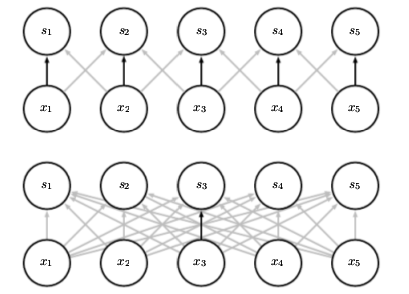
\includegraphics[scale=0.7]{fig/param_sharing}
\caption[Connections \gls{fnn} and \gls{cnn}]{In an FCN, all units between layers are connected to each other, but in a CNN the nodes are only connected by the nodes from its receptive field in the previous layer. This makes the number of connections considerably smaller. The weights are also equal for every connection set between input nodes.}
\label{fig:ps}
\end{figure}

\subsubsection*{Convolutional Layer Architecture}
Convolutional layers typically consist out of 3 main stages as shown in figure \ref{fig:cnn}. The input is fed into the convolutional stage, which executes the convolution operations. This is followed by a nonlinear transformation just as in section \ref{sec:nn}. The convolutional layer can be finalized by an optional pooling stage if the model is used for computer vision purposes. The output of the last stage is then the input is then fed into the next convolutional layer, making \gls{cnn}s a feedforward architecture.\\
Pooling is a method to introduce extra invariances by downsampling the information. Additional information can be found in the references, but this method is not from crucial importance to this master dissertation \cite{boureau11}.\\

\begin{figure}
\centering
\begin{tikzpicture}
% 1st column
\node[staterect] (n0_0) at (0,0) {Input};
\node[staterect] (n0_2) at (0,-2) {Convolutional Stage} edge[mainedge] (n0_0);
\node[staterect] (n0_4) at (0,-4) {Nonlinear Stage} edge[mainedge] (n0_2);
\node[staterect] (n0_6) at (0,-6) {Pooling Stage} edge[mainedge] (n0_4);
\node[staterect] (n0_8) at (0,-8) {Output} edge[mainedge] (n0_6);
\draw (-3,-1) rectangle (3,-7);
\node[scale=0.75] at (1.5,-7.25) {Convolutional Layer};

\end{tikzpicture}
\caption{Convolutional layer flow diagram}
\label{fig:cnn}
\end{figure}

\subsection{Deep learning}
\label{subsubsec:dl}
Deep learning algorithms are (as the name suggests) neural networks using an architecture with many hidden layers. The conditions for an architecture to be 'deep' are that \cite{deng14}:
\begin{itemize}
\item it is a composition of successive layers, using the output of previous layer as input
\item it is based on hierarchical learning of feature representations of the data. The features learned in deeper layers are more complex and are derived from the low level features learned in earlier stages of the network.
\item learn multiple representations on different abstractions
\end{itemize}

\section{(Deep) Reinforcement Learning}
\label{sec:rl}

Just like neural networks are inspired by the functioning of the brain, \gls{rl} is a field in machine learning inspired by behaviorist psychology. The principal idea of solving problems in \gls{rl} is to find from any given situation in an environment the optimal sequence of actions such that an agent in the environment maximizes its reward. The bigger the rewards, the closer the agent is to achieving its final goal. The agent has to find this sequence by exploring the environment, where actions in given states lead to certain rewards. To better understand the environment and increase future rewards, the agent has to balance between exploiting current knowledge and exploring new areas of the environment where he knows less about, this is the exploration-exploitation dilemma. \\

\begin{figure}
\centering
\begin{tikzpicture}
\node[staterect] (n0_0) at (0,0) {Agent} edge[mainedge, bend left] (n0_4);
\node[staterect] (n0_4) at (0,-4) {Environment: $s_t$} edge[mainedge, bend left] (n0_0);
\node at (-1,-2) {$a_t$};
\node at (1.1,-2) {$r_{t+1}$};
\node at (1.1,-2.5) {$s_{t+1}$};
\end{tikzpicture}
\caption[\gls{rl} paradigm]{The general framework for \gls{rl}, an agent is performing an action $a_t$ in state $s_t$. By doing this action, it will receive its new state $s_{t+1}$ with the reward $r_{t+1}$ corresponding to the action at the next time step.}
\label{fig:rl}
\end{figure}

We start of this section with an explanation about Markov decision processes, the mathematical framework used for studying \gls{rl}. We will find out that for an agent to interpret its environment better, it should sense which states are best to reside in. Background on these problems are provided in section \ref{subsec:vp}. Similarly, we want to know which actions the agent should take to understand its environment to the best of his powers, this is examined in \ref{subsec:control}. This section is concluded with algorithms using value prediction as well as control in section \ref{subsec:iter}.

\subsection{Markov Decision Process}

Notations are inspired on the survey \textit{Algorithms for Reinforcement Learning} \cite{szepe10}.
\label{subsec:mdp}
\begin{definition}
An \gls{mdp} is a 5-tuple $\mathcal{M}=(\mathcal{S,A,P},R,\gamma)$ with
\begin{itemize}
\item $\mathcal{S}$: state space
\item $\mathcal{A}$: action space
\item $\mathcal{P}: \mathcal{S} \times \mathcal{A} \times \mathcal{S} \mapsto \mathbb{R} $: state transition probability kernel
\item $R: \mathcal{S} \times \mathcal{A} \mapsto \mathbb{R} $: the expected immediate reward function
\item $\gamma \in \mathbb{R} \cap (0,1) $: discount factor
\end{itemize}
\end{definition}

With \gls{mdp}s we can define sequential decision making problems in \gls{rl} as follows. Suppose $t \in \mathbb{N}$ denotes an instant of time, and we interact according \gls{mdp} $\mathcal{M}$. When an agent chooses action $a_t \in \mathcal{A}$ in state $s_t \in \mathcal{S}$, it gets fed back a reward $r_{t+1}$ and arrives in a new state $s_{t+1}$ with a probability $P(s_{t+1}|s_t,a_t)$. The expected reward at time step $t$ was $R(s_t,a_t)$, but from now on we assume this reward to be deterministic given $a_t$ and $s_t$ to simplify the framework. \\
From this point on, the same decision process goes on and on until the agent arrives at a terminal state $s_T$. A full sequence $\{s_1,s_2,\dotso,s_T\}$ is called an episode. The goal of the agent is to maximize its return over the course of an episode. The return starting from $t$ is defined as the exponentially discounted sum of the rewards obtained:
\begin{equation}
\mathcal{R}=\sum_{t=0}^{\infty}\gamma^t r_{t+1}
\end{equation}
In this manner, MDPs can balance between being discounted ($\gamma<1$) and undiscounted ($\gamma=1$).
The agent bases its future behavior on the history up until we arrived at $s_t$ is defined by the sequence of tuples $(s_0,a_0,r_1),(s_1,a_1,r_2), \dotso , (s_{t-1},a_{t-1},r_t)$. \\
From this point on, we will assume the \gls{mdp} to be deterministic, i.e. only one state transition $s_{t+1}$ is possible given $(s_t,a_t)$. To formally describe this, define the successor function $\Sigma: \mathcal{S} \times  \mathcal{A} \mapsto \mathcal{S}$. The state transition probability kernel simplifies to
\begin{equation}
P(s_{t+1}|s_t,a_t) = \left\{
  \begin{array}{ll}
    1 & \Sigma(s_t,a)=s_{t+1}\\
    0 & else
  \end{array}
\right.
\label{eq:det}
\end{equation} 

In the next chapter, we will see how chess can easily fit into this framework of \gls{mdp}s as a tool to learn to play chess.

\subsubsection*{Value Function}
Before we continue, we define the concept of a policy.
\begin{definition}
A policy is a probability function $\pi:\mathcal{S} \times \mathcal{A} \mapsto \mathbb{\mathbb{R}}$. An agent is following a policy $\pi$ if it draws its next action $a \in \mathcal{A}$ in state $s \in \mathcal{S}$  randomly with probability $\pi(a|s)$
\end{definition}
To find the optimal behavior in an \gls{mdp}, value functions are used. Value functions denote how good it is for an agent to be in certain states. For chess boards, this is equivalent to the static evaluation function.
\begin{definition}
The value function $V^{\pi}:\mathcal{S}\mapsto\mathbb{R}$ with underlying policy $\pi$ is defined by
\begin{equation}
V^{\pi}(s) = \mathbb{E}\left[\mathcal{R}|s\right] = \mathbb{E}\left[\sum_{t=0}^{\infty}\gamma^t r_{t+1}|s\right]
\label{eq:v}
\end{equation}
with the understanding that all triplets $(s_t,a_t,r_{t+1})$ came up by following $\pi$.
\end{definition}

In contrast to value functions, action value functions stand for the profit achieved by performing an action in a certain state.

\begin{definition}
The action value function $Q^{\pi}:\mathcal{S} \times \mathcal{A} \mapsto\mathbb{R}$ with underlying policy $\pi$ is defined by
\begin{equation}
Q^{\pi}(s,a) = \mathbb{E}\left[\mathcal{R}|s,a\right] = \mathbb{E}\left[\sum_{t=0}^{\infty}\gamma^t r_{t+1}|s,a\right]
\end{equation}
with the understanding that all triplets $(s_t,a_t,r_{t+1})$ came up by following $\pi$.
\end{definition}

An optimal policy can be derived easily supposing we have found the optimal value for every state in the state space, which is the highest achievable return starting from a state. The optimal value function $V^*:\mathcal{S}\mapsto\mathbb{R}$ attains this most favorable mapping. We define the optimal action value function $Q^{*}:\mathcal{S} \times \mathcal{A}$ analogously. The policy performing greedy actions only with respect to $Q^*$ is an optimal policy. As we can relate $V^*$ and $Q^*$ to each other by the coming equations:

\begin{align}
V^*(s) &= \max_{a \in A} Q^*(s,a) \\ 
Q^*(s,a) &= R(s,a) + \gamma V^*(\Sigma(s,a))
\end{align}

we can also act optimally according to $V^*$ by acting greedily with respect to the next state's value function.\\

The remaining question is now on how to find these optimal functions. A tool used for this are the recursive Bellman equations \cite{bert07}.
\begin{theorem}
The optimal value function satisfies
\begin{equation}
V^*(s) = \max_{a \in A} \left\{R(s,a) + \gamma V^*(\Sigma(s,a))\right\}
\end{equation}
The optimal action value function satisfies
\begin{equation}
Q^*(s,a) = R(s,a) + \gamma \max_{a'\in \mathcal{A}} Q^*(\Sigma(s,a),a')
\end{equation}
\end{theorem}

\subsection{Value Prediction}
\label{subsec:vp}

\subsubsection*{Monte Carlo method}
Let us consider the problem of the estimation of the value function. The closer we can approach the optimal value function with our estimate, the better our policy will be. We defined the value function earlier as the expected return starting from a certain state \ref{eq:v}. This definition gives us the insight that a possible algorithm to create approximations might be a Monte Carlo algorithm, averaging out all returns.\\
Suppose we have got an \gls{mdp} $\mathcal{M}=(\mathcal{S,A,P},R,\gamma)$ that generated $N$ episodes following a certain policy, with each episode having an index $n$ and history \[H_n=\left\{(s_0,a_0,r_1),(s_1,a_1,r_2), \dotso , (s_{T_{n}-1},a_{T_{n}-1},r_{T_{n}})\right\}\] Store the observed returns for every state in time in every episode
\begin{equation}
\mathcal{R}_n(t)=\sum_{t'=t}^{T_{n}-1}\gamma^{t'-t} r_{t'+1}
\end{equation}
We can now sensibly update the value function after the termination of an episode with a gradient descent kind of optimization step with the following update function
\begin{equation}
\hat{V}(s_t) \leftarrow \hat{V}(s_t)+\alpha\left(\mathcal{R}_n(t)-\hat{V}(s_t)\right)
\end{equation}
where $\alpha$ is the learning rate and $\mathcal{R}_n(t)-\hat{V}(s_t)$ is the gradient of the \gls{mse} between the actual observed return and the estimated return. We can find a nice recursive relationship between observed returns in an episode:
\begin{align*}
\mathcal{R}_n(T-1) &= r_{T} \\
\mathcal{R}_n(t)&= r_{t+1}+\gamma \mathcal{R}_n(t+1)
\end{align*}
This recursive relation is used in Algorithm \ref{al:evmc}, where the history of an episode is interpreted to update the value function. The presented algorithm is called the \gls{evmc} algorithm. At the moment, we are assuming tabular methods, where the value function is stored for each distinct state independently in an array.

\begin{algorithm}
\begin{algorithmic}
\REQUIRE $H=\left\{(s_0,a_0,r_1),(s_1,a_1,r_2), \dotso , (s_{T_{n}-1},a_{T-1},r_{T})\right\},V(s)$
\STATE $\mathcal{R}_n \leftarrow 0$
\FOR{$t \leftarrow T-1$ \textbf{downto} $ 0$}
\STATE $\mathcal{R}_n \leftarrow r_{t+1}+\gamma \mathcal{R}_n$
\STATE $V(s_t) \leftarrow V(s_t)+\alpha\left(\mathcal{R}_n-V(s_t)\right)$
\COMMENT{Gradient Descent update step}
\ENDFOR 
\end{algorithmic}
\caption{Episodical EMVC}
\label{al:evmc}
\end{algorithm}

In practice, \gls{evmc} stabilizes for the tabular method (which is only feasible for a limited amount of states) almost surely to the optimum. The issue is the variance between the calculated returns over episodes, which can be very high because we take every visited state into account (this is a general problem of \gls{mc} simulations in general \cite{robert05}), resulting in poor estimates at first and a long training time. \\

\subsubsection*{TD(0)}
To address the issues of \gls{evmc}, we will limit the influence of states further away in the episode with temporal difference learning, the most drastic one being TD(0), where we only use the value of the next state in our estimate. As in \gls{evmc}, we will use an online gradient descent algorithm. The update function is now (under the same \gls{mdp} conditions as in the MC method described earlier)
\begin{equation}
\hat{V}(s_t) \leftarrow \hat{V}(s_t)+\alpha\left(r_{t+1}+\gamma\hat{V}(s_{t+1}) -\hat{V}(s)\right)
\end{equation}
So basically, we have slightly modified the target for a state to a linear approximation of the true return in the episode. The TD-error is $r_{t+1}+\gamma\hat{V}(s_{t+1}) -\hat{V}(s)$. States further away than the next state do not influence the target anymore. These were exactly the states entailing the largest amount noise in \gls{mc} measurements. Another advantage over \gls{evmc} is its suitability for incremental learning, meaning we can update our value function after every action, as in algorithm \ref{al:td0}.

\begin{algorithm}
\begin{algorithmic}
\REQUIRE $s_t,r,s_{t+1},V$
\STATE $V(s_t) \leftarrow V(s_t)+\alpha\left(r_{t+1}+\gamma V(s_{t+1}) -V(s_t)\right)$
\COMMENT{gradient descent update step}
\end{algorithmic}
\caption{TD(0)}
\label{al:td0}
\end{algorithm}

Just like \gls{evmc}, TD(0) converges almost surely to $V^*$. One may wonder which algorithm works best and in which cases, as they both have their own merits. An example where TD(0) is slower than \gls{evmc} is a long chain of states where the agent only gets a positive reward at the final action, because the TD-error has to propagate back to the first states. So the longer the chain, the longer it will take until the initial states have learned which paths to follow.

\subsubsection*{TD($\lambda$)}
The attentive reader may have wondered why temporal difference learning is called TD(0). The reason behind the zero in the name is because it is actually a special case of TD($\lambda$), an algorithm unifying \gls{evmc} and TD(0). First of all, let us define the $n$-step return, which is a prediction of the actual return taking $n$ states ahead into account.
\begin{equation}
\label{eq:nstep}
G_n(t)=\left(\sum_{i=0}^{n-1}\gamma^i r_{t+i}\right)+\gamma^n V(s_t+n)
\end{equation}
We notice $G_1(t)$ to be the target return in TD(0) and $G_{T-t}(t)$ the real return value given $T$, the length of the episode. We construct the $\lambda$-return with all n-step returns with exponential decay as mixing weights.
\begin{equation}
\label{eq:tdlambda_inf}
G_{\lambda}(t)=(1-\lambda) \sum_{n=1}^{\infty} \lambda^{n-1}G_n(t)
\end{equation}
where it can easily be checked that $(1-\lambda)$ is a normalization factor. $\lambda$ is the trace decay parameter, and controls to what extent the algorithm resembles on TD(0) or a Monte Carlo algorithm. $\lambda=0$ gives TD(0). The finite version of equation \ref{eq:tdlambda_inf} is
\begin{equation}
\label{eq:tdlambda_fin}
G_{\lambda}(t)=(1-\lambda) \sum_{n=1}^{T-t} \lambda^{n-1}G_n(t) + \lambda^{T-t} G_t
\end{equation}
where we define $G_t$ to be all the subsequent $n$-step returns after the terminal state. \\
An incremental algorithm can be designed by using accumulating eligibility traces, which can be seen as some sort of history of past states. The TD-error propagates back to all past states when the incremental update occurs. Suppose $z$ is the eligibility trace, appropriate incremental updates are then \cite{sutton98}
\begin{align}
z(s_t) &\leftarrow 1+\gamma \lambda z(s_t) \\
V(s_t) &\leftarrow V(s_t)+\alpha\left(r_{t+1}+\gamma V(s_{t+1}) -V(s_t)\right)z(s_t)
\end{align}
Algorithm \ref{al:tdy_tab} gives pseudocode for a tabular TD($\lambda$) algorithm 

\begin{algorithm}
\begin{algorithmic}
\REQUIRE{$s_t, r_{t+1}, s_{t+1}, V, z$}
\FOR{$s \in \mathcal{S}$}
%\COMMENT{it is only necessary to look at the states in history episode}
\STATE{$z(s) \leftarrow \gamma \lambda z(s) + \mathbbm{1}_{\{s=s_t\}}$}
\STATE{$V(s) \leftarrow V(s)+\alpha\left(r_{t+1}+\gamma V(s_{t+1}) -V(s_t)\right)z(s_t)$ }
\ENDFOR
\end{algorithmic}
\caption{Tabular TD($\lambda$)}
\label{al:tdy_tab}
\end{algorithm}

In summary, TD($\lambda$) tries to assemble the advantages of both TD-learning and Monte Carlo methods. Just as these algorithms, it converges to $V^*$. Finding the right value of $\lambda$ for quicker convergence is often a process of trial and error, and it has even been proved that changing $\lambda$ during training does not impact convergence under the right circumstances (eg. eligibility trace update function) \cite{bert96}.

\subsubsection*{Function approximation}
The methods considered so far consider a tabular value function, but many problems like chess have such a large state space that saving all their values is infeasible. We choose to describe all states with feature vectors. A state $s \in \mathcal{S}$ is transformed to its feature vector of dimension $D$ by a feature extraction method $\phi: \mathcal{S} \mapsto \mathbb{(R)}^D$. The value function can then be constructed around a mathematical model operating on these feature vectors $\phi(s)$. This model introduces a new set of parameters, the weights $w$ of the model. \\
Some examples of function approximation methods are
\begin{itemize}
\item linear: $V_w(s)=w^T \phi(s)$
\item neural networks (see Section \ref{sec:nn})
\item other mathematical models for machine learning 
\end{itemize}

Deep \gls{rl} is the class of \gls{rl} algorithms using deep neural networks as function approximation method. From now on it is assumed neural networks are used for this task. The tabular methods we have discussed so far now needs to be generalized to algorithms with function approximation. As Monte Carlo algorithms and TD(0) can be seen as special cases of TD($\lambda$), we will limit our examination to TD($\lambda$). An example of a non incremental episodic learning algorithm works as follows:
\begin{enumerate}
\item run episode and get history $\mathcal{H}_n$
\item calculate the $\lambda$-returns for all states in $\mathcal{H}_n$
\item use the $\lambda$-returns as target values for supervised learning on a neural network.
\item update weights of neural network with gradient descent 
\end{enumerate} 
As we want to learn a continuous value function, this is a regression problem. A classical loss function to optimize in regression problems is the Mean Squared Error (MSE): $L_w(\hat{V},V)=(\hat{V}-V)^2/2$. \\
When using non-linear value function approximators, convergence is no longer guaranteed \cite{baird95}.However, the algorithm generally still finds good results in practice  under the right choice of hyper-parameters.

\subsection{Control}
\label{subsec:control}
We primarily focus on learning problems where the agent can influence its observations, which is interactive learning. The agent is making decisions changing the state of the environment and improving its policy. There are two ways for the agent to improve its policy. It can use active learning, where it will control the samples such that it maximizes finding a good policy or it can use online learning, where the online performance is optimized.

\subsubsection{Closed-loop Online Learning}
\label{subsec:clil}
It is from crucial importance in online learning to occasionally choose  actions that at the time might look suboptimal, to augment the future payoff. This question is then how frequent the agent must balance its choice to explore or exploit the current environment. This means that the methods described in this section can be used independently from which value functions are used. \\

\textbf{$\epsilon$-greedy policy}
This is a very simple strategy to balance exploitation and exploration, choose a fixed parameter $\epsilon \in \mathbb{R} \cap [0,1]$ and at every state choose a random action with probability $\epsilon$. Although this method is really simple, it can be competitive with more sophisticated algorithms if we some time decay is employed and tuned. Time decay is beneficial as normally the policy should improve, hence we should exploit more as time goes on. \\

\textbf{Boltzmann exploration strategy}
With $\epsilon$-greedy, actions are drawn uniformly with a probability $\epsilon$. We may want to draw seemingly worse actions with a lower probability. To attain this property, we can use the distribution
\begin{equation}
\pi(a|s)=\frac{e^{\beta J(s,a)}}{\sum_{a' \in \mathcal{A}_s} e^{\beta J(s,a)}}
\end{equation}
$\beta$ controls how greedy the action will be, while $J: \mathcal{S} \times \mathcal{A} \mapsto \mathbb{R}$ is a function indicating how good the action is, like $V(\Sigma(s))$ or $Q(s,a)$. 

\subsubsection{Q-learning}
By trying to learn $Q^*$ immediately, a greedy policy may be close to optimal.

With tabular Q-learning, an estimate for every $(s,a)$-tuple is stored and updated incrementally. Just as in TD-learning, this update happens in a gradient descent manner, by moving the Q-value in the direction of the last error between the target and previous estimate. Upon the observation of $(s_t,a_t,r_{t+1},s_{t+1})$, the Q-value changes to
\begin{equation}
Q(s_t,a_t) \leftarrow Q(s_t,a_t)+\alpha \left(r_{t+1}+\gamma \max_{a' \in \mathcal{A}} \left\{ Q(s_{t+1},a')\right\}-Q(s_t,a_t)\right)
\end{equation}
Analogous to TD-learning, the target value of our estimate is $r_{t+1}+\gamma \max_{a' \in \mathcal{A}} \left\{ Q(s_{t+1},a')\right\}$. \\
Q-learning is very attractive due to its simplicity, and its convergence to $Q^*$. The policy followed by the agent could be $\epsilon$-greedy or \textit{Boltzmann} exploration. \\
Incremental Deep Q-learning algorithms can then be generated with the extension to function approximation for $Q_w$:
\begin{equation}
w \leftarrow w+\alpha \left(r_{t+1}+\gamma \max_{a' \in \mathcal{A}} \left\{ Q_w(s_{t+1},a')\right\}-Q_w(s_t,a_t)\right) \nabla_w Q_w(s_t,a_t)
\end{equation}
This update rule is used plenty of times in practice. However, its convergence properties are doubtful to say at least, especially when non linear approximation methods like deep learning are used. \\

Analogous to our deep TD($\lambda$) algorithm, we can use episodic experience to learn the optimal weights of our network with regression. Good empirical results have been obtained by adding new samples to the data used for the previous iteration \cite{ried05}.

\subsection{Value and Policy Iteration}
\label{subsec:iter}
The presented Q-learning and TD-learning algorithms are value iteration algorithms, by exploring the environment the value function changes up until the point it has converged. There are two weaknesses to applying value iteration only:
\begin{itemize}
\item may take a long time to converge
\item we actually try to find the optimal policy, the value function is just a tool to do so
\end{itemize}
To incorporate the updates of policies, we can iterate over value iteration and policy iteration.
\begin{enumerate}
\item pick a random policy $\pi$
\item update $V^{\pi}$ under the policy
\item improve $\pi$
\item go back to step 2 if satisfied
\end{enumerate}
We actually already discussed a value and policy iteration algorithm, namely the use of the \textit{Boltzmann} distribution to choose the next action. In that example, we updated the policy in an incremental fashion, as there is an immediate relationship between the policy and the value function.
